\chapter{路径构建}
路径包括构建路径,以及路径操作。本章主要讲解构建这一部分。\texinline{\path (0,0) --
	(1,1);}会新建一条路径,但是表面上看不到什么变化。路径的操作要将操作的内容放置在\texinline{[]}中,比如\\\texinline{\path[draw]
	(0,0) -- (1,1);},而我们平时用的\texinline{\draw}命令其实只是\texinline{\path[draw]}的快捷方式。
\section{移动 Move-To}
这个操作就像是提着笔移动到一个位置,但是没有下笔画任何内容。
\begin{texlst}
	\begin{tikzpicture}
		\draw (0,0) -- (2,0) (0,1) -- (2,1);
	\end{tikzpicture}
\end{texlst}
上面的例子中先是移动到\texinline{(0,0)},然后下笔画到\texinline{(2,0)};接下来移动到\texinline{(0,1)},再下笔画到\texinline{(2,1)}。
其中的\texinline{--(2,0)}和\texinline{--(2,1)}这个操作称为画线操作(line-to)。

有一个特殊的坐标称之为\texinline{current subpath start}, 这个值永远是最后一个移动操作的坐标。如下例:
\begin{texlst}
	\tikz[line width=2mm]
	\draw (0,0) -- (1,0) -- (1,1) -- (0,1) -- (current subpath start);
\end{texlst}

\section[直线连接符]{直线连接符\tt{--}}
这个是最常用的,与此操作符类似的还有\texinline{to}和\texinline{edge},\texinline{--}是最简单的,无法搭配选项使用。

注意,在需要图形实现闭包的情况下,最后需要用\texinline{cycle}来代替初始点。否则接头的地方实现不是完美的接合。

\section[直角连接符]{直角连接符\tt{|-}\quad、\tt{-|}}
这两个操作符使用起来非常直观。
\begin{texlst}
	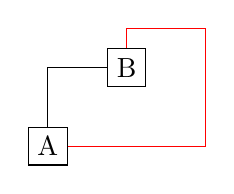
\begin{tikzpicture}
		\draw (0,0) node (a) [draw] {A} (1,1) node(b) [draw] {B};

		\draw (a.north) |- (b.west);
		\draw [color=red] (a.east) -| (2,1.5) -| (b.north);
	\end{tikzpicture}
\end{texlst}

\section{曲线连接符 .. controls a and b ..}
曲线连接所控制的两个点分别与起点和终点正切,如果只提供一个控制点,则认为第二个控制点与第一个相同。
\begin{texlst}
	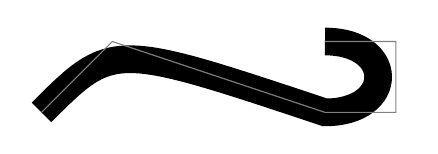
\begin{tikzpicture}[scale=0.9]
		\draw[line width=10pt] (0,0) .. controls (1,1) .. (4,0) .. controls (5,0) and (5,1) .. (4,1);
		\draw[color=gray] (0,0) -- (1,1) -- (4,0) -- (5,0) -- (5,1) -- (4,1);
	\end{tikzpicture}
\end{texlst}

\section{矩形 rectangle}
绘制矩形比较简单,只需要提供两个对角的点坐标即可。
\begin{texlst}
	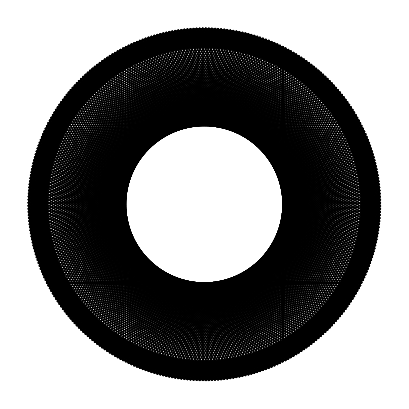
\begin{tikzpicture}
		\foreach \a in {0,1,...,360}
		\draw [rotate=\a] (-2,-1) rectangle (2,1);
	\end{tikzpicture}
\end{texlst}
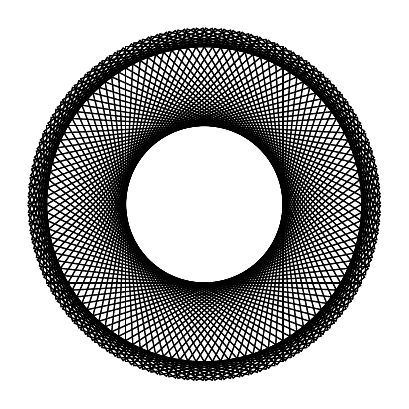
\begin{tikzpicture}
	\foreach \a in {0,3,...,360}
	\draw [rotate=\a] (-2,-1) rectangle (2,1);
\end{tikzpicture}
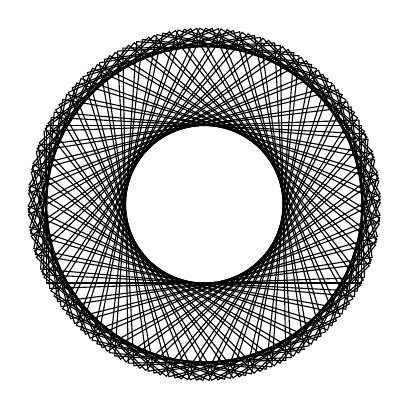
\begin{tikzpicture}
	\foreach \a in {0,7,...,360}
	\draw [rotate=\a] (-2,-1) rectangle (2,1);
\end{tikzpicture}
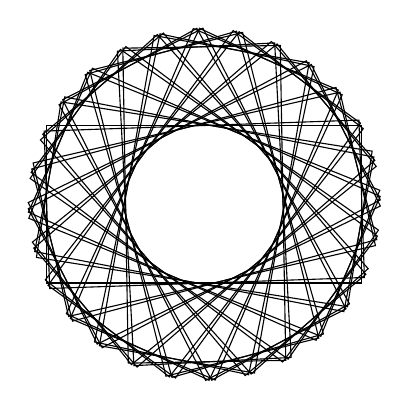
\begin{tikzpicture}
	\foreach \a in {0,13,...,360}
	\draw [rotate=\a] (-2,-1) rectangle (2,1);
\end{tikzpicture}

以上三个图形是分别按3、7、13的角度偏转矩形时产生的。

\section{圆角 rounded corners}
\texinline{rounded corners}命令的默认值是\texinline{4pt},角的形状默认是\texinline{sharp corners}。

\section{圆形和椭圆 circle ellipse}
这两个命令是一样的,不过我还是习惯画圆的时候用\texinline{circle},而画椭圆的时候用\texinline{ellipse}。
\begin{texlst}
	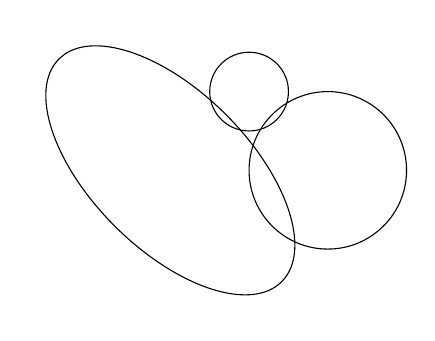
\begin{tikzpicture}[every circle/.style={fill}]
		\draw [x radius=1, y radius=2, rotate=45] circle;
		\draw (2,0) ellipse [radius=1];
		\draw (1,1) circle (0.5);
	\end{tikzpicture}
\end{texlst}
可以看到\texinline{every circle/.style}是不起作用的,我查看了一个,\tikzname 其实提供了\\
\texinline{every circle node/.style},当然,其中的\texinline{circle}也可以是其他的形状。

\section{圆弧 arc}
圆弧一般都会提供\texinline{start angle}和\texinline{end angle},另外还有一个\texinline{delta angle}。如果\texinline{end
	angle}为空,则用\texinline{start angle}加上\texinline{delta angle}来代替。如果\texinline{start angle}为空,则用\texinline{end
	angle}减去\\\texinline{delta angle}来代替。若三者都提供了\texinline{delta angle}不起任何作用。
\begin{texlst}
	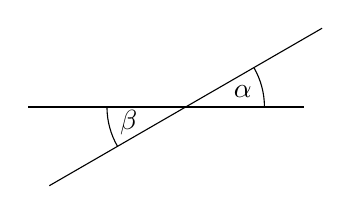
\begin{tikzpicture}[radius=1cm, delta angle=30]
		\draw (-1,0) -- +(3.5,0);
		\draw (1,0) ++(210:2cm) -- +(30:4cm);
		\draw (1,0) +(0:1cm) arc [start angle=0];
		\draw (1,0) +(180:1cm) arc [start angle=180];
		\path (1,0) ++(15:.75cm) node{$\alpha$};
		\path (1,0) ++(15:-.75cm) node{$\beta$};
	\end{tikzpicture}
\end{texlst}
\emph{注意:}不能用\texinline{\node (1,0)+(0:1cm) {text};},而要使用上面代码段中的\texinline{\path}语法。

\section{网格grid}
\texinline{grid}一般用来画参照线,对应的有\texinline{help
	lines}的预设样式,另外还可以用\texinline{step}\texinline{xstep}\texinline{ystep}来设置步长。

\section{抛物线 parabola}
这个我目前还没有用到过,先占个坑,看以后是不是会有需求。
\begin{texlst}
	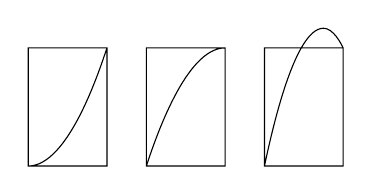
\begin{tikzpicture}
		\draw (0,0) rectangle (1,1.5)
		(0,0) parabola (1,1.5);
		\draw[xshift=1.5cm] (0,0) rectangle (1,1.5)
		(0,0) parabola[bend at end] (1,1.5);
		\draw[xshift=3cm] (0,0) rectangle (1,1.5)
		(0,0) parabola bend (.75, 1.75) (1,1.5);
	\end{tikzpicture}
\end{texlst}

另外还有\texinline{bend pos}来设置拐点的比例位置,另外还有\texinline{parabola height}用来设置抛物线的高度。
\begin{texlst}
	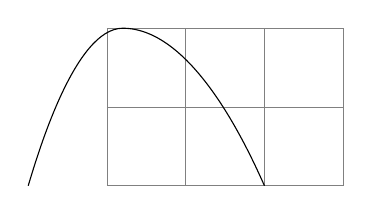
\begin{tikzpicture}
		\draw [help lines] (0,0) grid (3,2);
		\draw (-1,0) parabola[bend pos=0.4] bend +(0,2) +(3,0);
	\end{tikzpicture}
\end{texlst}

\section{正弦和余弦曲线 Sin Cos}
两点之间的连接曲线是$[0, \pi/2]$的正弦曲线,会根据距离缩放和偏移。

\section{SVG}
这个没有学过,就不往里面跳了。

\section{Plot}
这个会在后面专门讲。

\section{To 操作符}
这个在讲直线连接符的时候提到过,与\texinline{--}只能绘制直线不一样,\texinline{to}操作符可以带很多选项来实现路径形状的变化。

在\texinline{to}构建的路径形成之前,\texinline{\tikztostart}、\texinline{\tikztotarget}和\texinline{\tikztonodes}会被设定,内容从名字上就可以推断出来了。

有了这几个宏就可以实现一些方便的操作,比如:
\begin{texlst}
	\begin{tikzpicture}[skip loop/.style={to path={-- +(0,0.5) -| (\tikztotarget) \tikztonodes}, -Stealth,shorten >=1pt,
					draw=black!50, thick, rounded corners}]
		\draw (-1,0) -- (3,0);
		\draw[skip loop] (0,0) to (2,0);
	\end{tikzpicture}
\end{texlst}

\begin{texlst}
	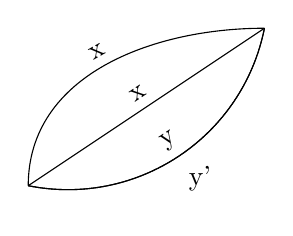
\begin{tikzpicture}
		\draw (0,0) to node [sloped, above] {x} (3,2);
		\draw (0,0) to [out=90, in=180] node [sloped, above] {x} (3,2);
		\draw (0,0) to [bend right=45] node [sloped, above] {y} (3,2);
		\draw (0,0) to [bend right=45, edge label'=y'] (3,2);
	\end{tikzpicture}
\end{texlst}

一些具体的路径变化命令,比如\texinline{bend
	right}等这一节里面都没有讲到,这一章主要是讲路径的构造方式,所以细节这里暂时略过。
另外还有一个\texinline{every to}可以设置全局的\texinline{to}样式。

\section{循环命令foreach}
这个命令我比较熟练了,之前在讲矩形路径构造的时候已经动手写过了。

\section{Let赋值命令}
\texinline{\let}命令需要加载\texinline{calc}库。用一个示例来记录一下用法吧。
\begin{texlst}
	\begin{tikzpicture}
		\draw [help lines] (0,0) grid (3,3);

		\coordinate (a) at (rnd, rnd);
		\coordinate (b) at (3-rnd, 3-rnd);
		\draw (a) -- (b);

		\node (c) at (1,2) {x};

		\draw let \p1 = ($(a)!(c)!(b) - (c)$),
		\n1 = {veclen(\x1, \y1)}
		in circle [at=(c), radius=\n1];
	\end{tikzpicture}
\end{texlst}
其中\texinline{\p}为点寄存器, \texinline{\n}为数值寄存器,\texinline{\x}、\texinline{\y}分别为$x$和$y$坐标寄存器。

\section{保存和使用路径Save Path \&\ Use Path}
\begin{texlst}
	\usetikzlibrary{intersections}
	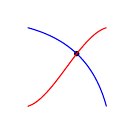
\begin{tikzpicture}
		\path[save path=\pathA, name path=A] (0,1) to [bend left] (1,0);
		\path[save path=\pathB, name path=B] (0,0) .. controls (.33, .1)
		and (.66, .9) .. (1,1);

		\fill [name intersections={of=A and B, by=p}] (p) circle (1pt);

		\draw[blue] [use path=\pathA];
		\draw[red] [use path=\pathB];

	\end{tikzpicture}

\end{texlst}
